
% \begin{figure}
%     \centering
%     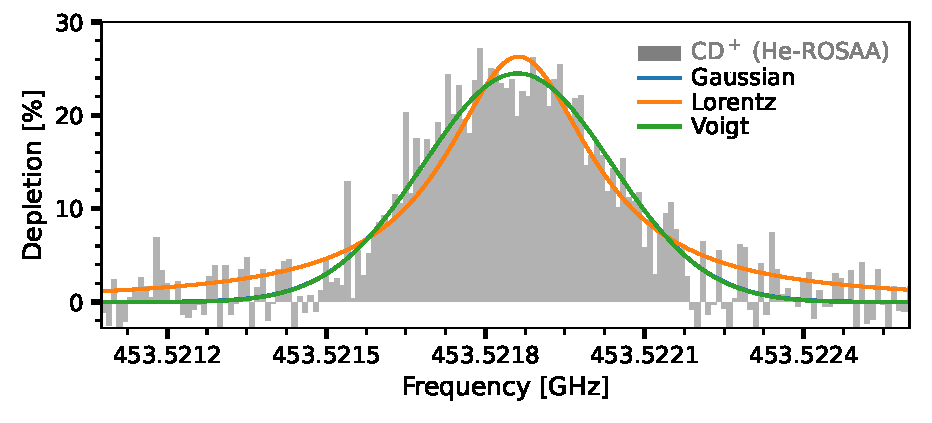
\includegraphics[width=1\textwidth]{figures/measurements/THz/thz_CD+_He.pdf}
%     \caption{\CD measured J$= 1-0$ rotational transition. The colored solid lines indicates the fitted line profile as labelled. The experiment performed at T$_{trap}=4.7(3)$K with He tag ROSAA technique (see Section \ref{subsec:ROSAA}) and derived T$_{ion} = 14(5)$K and T$_{coll} = 7(1)$K.}
%     \label{fig:thz:HeCD+}
% \end{figure}

% \begin{figure}
%     \centering
%     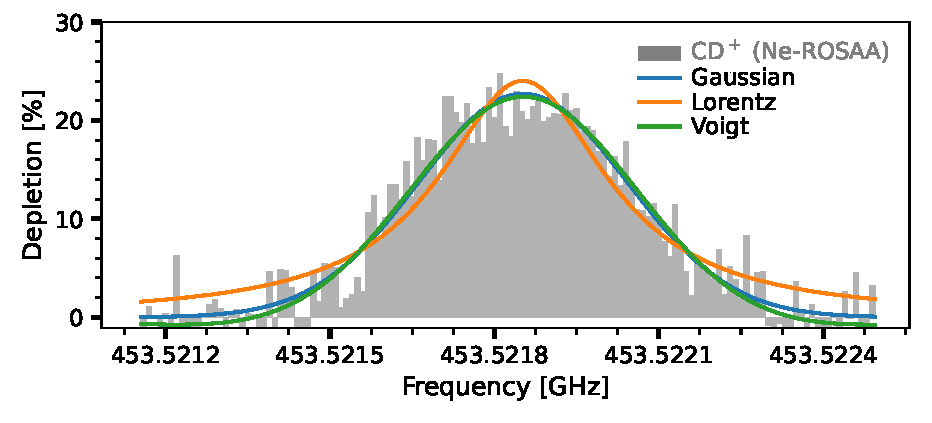
\includegraphics[width=1\textwidth]{figures/measurements/THz/thz_CD+_Ne.pdf}
%     \caption{\CD measured J$= 1-0$ rotational transition. The colored solid lines indicates the fitted line profile as labelled. The experiment performed at T$_{trap}=8.7(3)$K with He tag ROSAA technique (see Section \ref{subsec:ROSAA}) and derived T$_{ion} = 23(5)$K and T$_{coll} = 19(3)$K.}
%     \label{fig:thz:NeCD+}
% \end{figure}

\begin{figure}[!htb]
    \centering
    \begin{subfigure}[b]{0.49\textwidth}
        \centering
        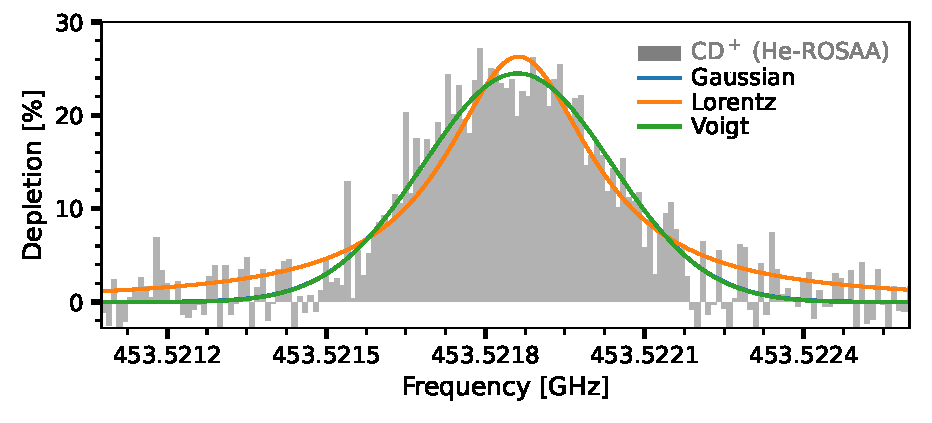
\includegraphics[width=1\textwidth]{figures/measurements/THz/thz_CD+_He.pdf}
        \caption{}
        \label{fig:thz:HeCD+}
    \end{subfigure}
    \hfill
    \begin{subfigure}[b]{0.49\textwidth}
        \centering
        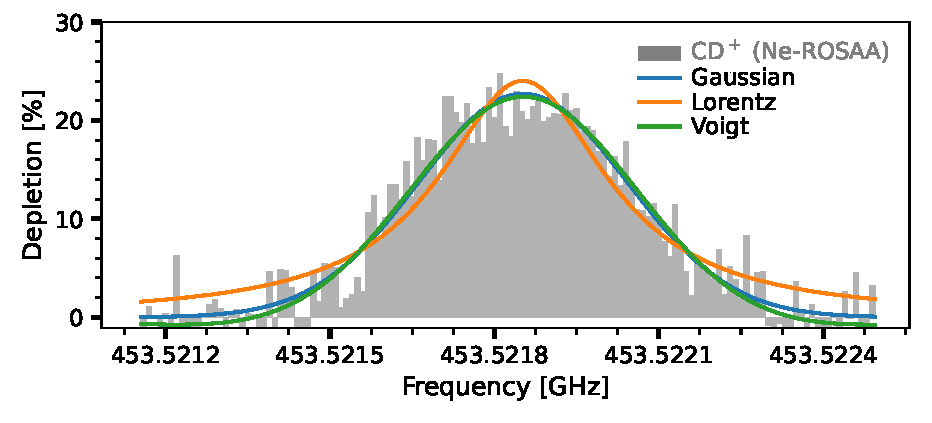
\includegraphics[width=1\textwidth]{figures/measurements/THz/thz_CD+_Ne.pdf}
        \caption{}
        \label{fig:thz:NeCD+}
    \end{subfigure}
    \caption{\CD measured \CDline rotational transition using ROSAA technique  (see Section \ref{subsec:ROSAA}). The coloured solid lines indicate the fitted line profile as labelled. The experiment performed at $35(12) \sim \mu$W power - (a) with He tag, T$_{trap}=4.7(3)$ K [$2.7(4) \cdot 10^{14}$ \percc] with He tag  and derived T$_{ion} = 14(5)$ K and T$_{coll} = 7(1)$ K; (b): with Ne tag , T$_{trap}=8.7(3)$ K [$1.8(2)\cdot 10^{14}$ \percc] and derived T$_{ion} = 23(5)$ K and T$_{coll} = 19(3)$ K.}
    \label{fig:thz}
\end{figure}